% !TEX root = saveliev_physics_general_course_2.tex
%!TEX TS-program = pdflatex
%!TEX encoding = UTF-8 Unicode


\chapter{ELECTRIC FIELD IN A VACUUM}\label{chap:1}

\section{Electric Charge}\label{sec:1_1}

All bodies in nature are capable of becoming electrified, \ie, acquiring an electric charge. The presence of such a charge manifests itself in that a charged body interacts with other charged bodies. Two kinds of electric charges exist. They are conventionally called positive and negative. Like charges repel each other, and unlike charges attract each other.

An electric charge is an integral part of certain elementary particles\footnote{Elementary particles are defined as such microparticles whose internal structure at the present level of development of physics cannot be conceived as a combination of other particles.}. The charge of all elementary particles (if it is not absent) is identical in magnitude. It can be called an \textbf{elementary charge}. We shall use the symbol $e$ to denote a positive elementary charge.

The elementary particles include, in particular, the electron (carrying the negative charge $-e$), the proton (carrying the positive charge $+e$), and the neutron (carrying no charge). These particles are the bricks which the atoms and molecules of any substance are built of, therefore all bodies contain electric charges. The particles carrying charges of different signs are usually present in a body in equal numbers and are distributed over it with the same density. The algebraic sum of the charges in any elementary volume of the body equals zero in this case, and each such volume (as well as the body as a whole) will be neutral. If in some way or other we create a surplus of particles of one sign in a body (and, correspondingly, a shortage of particles of the opposite sign), the body will be charged. It is also possible, without changing the total number of positive and negative particles, to cause them to be redistributed in a body so that one part of it has a surplus of charges of one sign and the other part a surplus of charges of the opposite sign. This can be done by bringing a charged body close to an uncharged metal one.

Since a charge $q$ is formed by a plurality of elementary charges, it is an integral multiple of $e$:
\begin{equation}\label{eq:1_1}
	q = \pm N e.
\end{equation}

\noindent
An elementary charge is so small, however, that macroscopic charges may be considered to have continuously changing magnitudes.

If a physical quantity can take on only definite discrete values, it is said to be quantized. The fact expressed by \eqn{1_1} signifies that an electric charge is quantized.

The magnitude of a charge measured in different inertial reference frames will be found to be the same. Hence, an electric charge is relativistically invariant. It thus follows that the magnitude of a charge does not depend on whether the charge is moving or at rest.

Electric charges can vanish and appear again. Two elementary charges of opposite signs always appear or vanish simultaneously, however. For example, an electron and a positron (a positive electron) meeting each other annihilate, \ie, transform into neutral gamma-photons. This is attended by vanishing of the charges $-e$ and $+e$. In the course of the process called the birth of a pair, a gamma-photon getting into the field of an atomic nucleus transforms into a pair of particles---an electron and a positron. This process causes the charges $-e$ and $+e$ to appear.

Thus, the total charge of an electrically isolated system\footnote{A system is referred to as electrically isolated if no charged particles can penetrate through the surface confining it.} cannot change. This statement forms the \textbf{law of electric charge conservation}.

We must note that the law of electric charge conservation is associated very closely with the relativistic invariance of a charge. Indeed, if the magnitude of a charge depended on its velocity, then by bringing charges of one sign into motion we would change the total charge of the relevant isolated system.

\section{Coulomb's Law}\label{sec:1_2}

The law obeyed by the force of interaction of point charges was established experimentally in 1785 by the French physicist Charles A. de Coulomb (1736-1806). A \textbf{point charge} is defined as a charged body whose dimensions may be disregarded in comparison with the distances from this body to other bodies carrying an electric charge.

Using a torsion balance (\fig{1_1}) similar to that employed by H. Cavendish to determine the gravitational constant (see Vol. I, Sec. 6.1), Coulomb measured the force of interaction of two charged spheres depending on the magnitude of the charges on them and on the distance between them. He proceeded from the fact that when a charged metal sphere was touched by an identical uncharged sphere, the charge would be distributed equally between the two spheres.

\begin{figure}[t]
	\begin{center}
		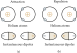
\includegraphics[scale=0.9]{figures/ch_01/fig_1_1.pdf}
		\caption[]{}
		\label{fig:1_1}
	\end{center}
	\vspace{-0.8cm}
\end{figure}

As a result of his experiments, Coulomb arrived at the conclusion that \textit{the force of interaction between two stationary point charges is proportional to the magnitude of each of them and inversely proportional
to the square of the distance between them}. The direction of the force coincides with the straight line connecting the charges.

It must be noted that the direction of the force of interaction along the straight line connecting the point charges follows from considerations of symmetry. An empty space is assumed to be homogeneous and isotropic. Consequently, the only direction distinguished in the space by stationary point charges introduced into it is that from one charge to the other. Assume that the force $\vec{F}$ acting on the charge $q_i$ (\fig{1_2}) makes the angle $\alpha$ with the direction from $q_1$ to $q_2$, and that $\alpha$ differs from $0$ or $\pi$. But owing to axial symmetry, there are no grounds to set the force $\vec{F}$ aside from the multitude of forces of other directions making the same angle $\alpha$ with the axis $q_1$-$q_2$ (the directions of these forces form a cone with a cone angle of $2\alpha$). The difficulty appearing as a result of this vanishes when $\alpha$ equals $0$ or $\pi$.

\begin{figure}[t]
	\begin{minipage}[t]{0.5\linewidth}
		\begin{center}
			
\includegraphics[scale=1]{figures/ch_01/fig_1_2.pdf}
			\caption[]{}
			\label{fig:1_2}
		\end{center}
	\end{minipage}
	\hfill{ }%\hspace{-0.1cm}
	\begin{minipage}[t]{0.5\linewidth}
		\begin{center}
			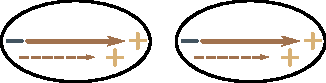
\includegraphics[scale=1]{figures/ch_01/fig_1_3.pdf}
			\caption[]{}
			\label{fig:1_3}
		\end{center}
	\end{minipage}
\vspace{-0.4cm}
\end{figure}

Coulomb's law can be expressed by the formula
\begin{equation}\label{eq:1_2}
	\vec{F}_{12} = -k \frac{q_1 q_2}{r^2}\,\vecuni{12}.
\end{equation}

\noindent
Here, $k$ is a proportionality constant assumed to be positive, $q_1$ and $q_2$ are magnitudes of the interacting charges, $r$ is the distance between the charges, $\vecuni{12}$ is the unit vector directed from the charge $q_1$ to $q_2$ and $\vec{F}_{12}$ is the force acting on the charge $q_1$ (\fig{1_3}; the figure corresponds to the case of like charges).

The force $\vec{F}_{21}$ differs from $\vec{F}_{12}$ in its sign:
\begin{equation}\label{eq:1_3}
	\vec{F}_{21} = k \frac{q_1 q_2}{r^2}\,\vecuni{12}.
\end{equation}

The magnitude of the interaction force, which is the same for both charges, can be written in the form
\begin{equation}\label{eq:1_4}
	F = k \frac{\absolute{q_1 q_2}}{r^2}.
\end{equation}

Experiments show that the force of interaction between two given charges does not change if other charges are placed near them. Assume that we have the charge $\ab{q}{a}$ and, in addition, $N$ other charges $q_1, q_2,\ldots, q_N$. It can be seen from the above that the resultant force $\vec{F}$ with which all the $N$ charges $q_i$ act on $\ab{q}{a}$ is
\begin{equation}\label{eq:1_5}
	\vec{F} = \sum_{i=1}^N \ab{\vec{F}}{a, $i$}
\end{equation}

\noindent
where $\ab{\vec{F}}{a, $i$}$ is the force with which the charge $q_i$ acts on $\ab{q}{a}$ in the absence of the other $N-1$ charges.

The fact expressed by \eqn{1_5} permits us to calculate the force of interaction between charges concentrated on bodies of finite dimensions, knowing the law of interaction between point charges. For this purpose, we must divide each charge into so small charges $\deriv{q}$ that they can be considered as point ones, use \eqn{1_2} to calculate the force of interaction between the charges $\deriv{q}$ taken in pairs, and then perform vector summation of these forces. Mathematically, this procedure coincides completely with the calculation of the force of gravitational attraction between bodies of finite dimensions (see Vol. I, Sec. 6.1).

All experimental facts available lead to the conclusion that Coulomb's law holds for distances from \SI{e-15}{\metre} to at least several kilometres. There are grounds to presume that for distances smaller than \SI{e-16}{\metre} the law stops being correct. For very great distances, there are no experimental confirmations of Coulomb's law. But there are also no reasons to expect that this law stops being obeyed with very great distances between charges.

\section{Systems of Units}\label{sec:1_3}

We can make the proportionality constant in \eqn{1_2} equal unity by properly choosing the unit of charge (the units for $F$ and $r$ were established in mechanics). The relevant unit of charge (when $F$ and $r$ are measured in cgs units) is called the \textbf{absolute electrostatic unit} of charge (cgse$_q$). It is the magnitude of a charge that interacts with a force of \SI{1}{\dyne} in a vacuum with an equal charge at a distance of \SI{1}{\centi\metre} from it.

Careful measurements (they are described in~\sect{10_3}) showed that an elementary charge is
\begin{equation}\label{eq:1_6}
	e = \num{4.80e-10}\text{ cgse$_q$}.
\end{equation}

Adopting the units of length, mass, time, and charge as the basic ones, we can construct a system of units of electrical and magnetic quantities. The system based on the centimetre, gramme, second, and the cgse$_q$ unit is called the \textbf{absolute electrostatic system of units} (the cgse system). It is founded on Coulomb's law, \ie, the law of interaction between charges at rest. On a later page, we shall become acquainted with the \textbf{absolute electromagnetic system of units} (the cgsm system) based on the law of interaction between conductors carrying an electric current. The Gaussian system in which the units of electrical quantities coincide with those of the cgse system, and of magnetic quantities with those of the cgsm system, is also an absolute system.

Equation~\eqref{eq:1_4} in the cgse system becomes
\begin{equation}\label{eq:1_7}
	F = \frac{\absolute{q_1 q_2}}{r^2}.
\end{equation}

\noindent
This equation is correct if the charges are in a vacuum. It has to be determined more accurately for charges in a medium (see \sect{2_8}).

USSR State Standard GOST 9867-61, which came into force on January 1, 1963, prescribes the preferable use of the International System of Units (SI). The basic units of this system are the metre, kilogramme, second, ampere, kelvin, candela, and mole. The SI unit of force is the newton (\si{\newton}) equal to \num{e5} dynes.

In establishing the units of electrical and magnetic quantities, the SI system, like the cgsm one, proceeds from the law of interaction of current-carrying conductors instead of charges. Consequently, the proportionality constant in the equation of Coulomb's law is a quantity with a dimension and differing from unity.

The SI unit of charge is the coulomb (\si{\coulomb}). It has been found experimentally that
\vspace{-12pt}
\begin{equation}\label{eq:1_8}
	\SI{1}{\coulomb} = \num{2.998e9} \approx \num{3e9}{\text{ cgse$_q$}}.
\end{equation}

To form an idea of the magnitude of a charge of \SI{1}{\coulomb}, let us calculate the force with which two point charges of \SI{1}{\coulomb} each would interact with each other if they were \SI{1}{\metre} apart. By \eqn{1_7}
\begin{equation}\label{eq:1_9}
	F = \frac{\num{3e9}\times\num{3e9}}{100^2}\,\text{ cgse$_F$} = \SI{9e14}{\dyne} = \SI{9e9}{\newton} \approx \SI{e9}{\kgf}.
\end{equation}

An elementary charge expressed in coulombs is
\begin{equation}\label{eq:1_10}
	e = \SI{1.60e-19}{\coulomb}.
\end{equation}

\section{Rationalized Form of Writing Formulas}\label{sec:1_4}

Many formulas of electrodynamics when written in the cgs systems (in particular, in the Gaussian one) include as factors $4\pi$ and the so-called electromagnetic constant $c$ equal to the speed of light in a vacuum. To eliminate these factors in the formulas that are most important in practice, the proportionality constant in Coulomb's law is taken equal to $1/4\pi\varepsilon_0$. The equation of the law for charges in a vacuum will thus become
\begin{equation}\label{eq:1_11}
	F = \frac{1}{4\pi\varepsilon_0}\frac{\absolute{q_1 q_2}}{r^2}.
\end{equation}

\noindent
The other formulas change accordingly. This modified way of writing formulas is called \textbf{rationalized}. Systems of units constructed with the use of rationalized formulas are also called \textbf{rationalized}. They include the SI system.

The quantity $\varepsilon_0$ is called the \textbf{electric constant}. It has the dimension of capacitance divided by length. It is accordingly expressed in units called the farad per metre. To find the numerical value of $\varepsilon_0$, we shall introduce the values of the quantities corresponding to the case of two charges of \SI{1}{\coulomb} each and \SI{1}{\metre} apart into \eqn{1_11}. By \eqn{1_9}, the force of interaction in this case is \SI{9e9}{\newton}. Using this value of the force, and also $q_1=q_2=\SI{1}{\coulomb}$ and $r=\SI{1}{\metre}$ in \eqn{1_11}, we get
\begin{equation*}
	\num{9e9} = \frac{1}{4\pi\varepsilon_0}\frac{\absolute{1\times 1}}{1^2}
\end{equation*}

\noindent
whence
\begin{equation}\label{eq:1_12}
	\varepsilon_0 = \frac{1}{4\pi\times\num{9e9}} = \SI{0.885e-11}{\faraday\per\metre}.
\end{equation}

The Gaussian system of units was widely used and is continuing to be used in physical publications. We therefore consider it essential to acquaint our reader with both the SI and the Gaussian system. We shall set out the material in the SI units showing at the same time how the formulas look in the Gaussian system. The fundamental formulas of electrodynamics written in the SI and the Gaussian system are compared in \app{A_3}.

\section{Electric Field. Field Strength}\label{sec:1_5}
